\documentclass[../Thesis-IJspeert.tex]{subfiles}

\begin{document}

\graphicspath{ {"Light Matter Interactions/figs/"} }
\pgfplotsset{table/search path={"Light Matter Interactions/data/"}}

\chapter{Light-Matter Interactions}
\addtocontents{toc}{\vskip-6pt\par\noindent\protect\textcolor{gray75}{\protect\rule{\textwidth}{0.5pt}}\par}
\label{chap:LightMatterInteractions}

%\subsection{Light-atom interactions}
The interaction of neutral atoms with a light field can be dissipative or conservative. The processes of absorption and spontaneous emission result in a net transfer of momentum, which gives rise to a dissipative scattering force that can be used for laser cooling and magneto-optical traps. The conservative part of the atom-light interaction stems from the fact that light induces a shift in the potential energy of the atom, which is known as the ac-Stark shift. If the light is far detuned from the atomic resonance, the rate of spontaneous emission is negligible. In this case, the energy shift can be used to establish a conservative trapping potential, which is the underlying mechanism of an optical dipole trap. After a brief discussion of the light-matter system Hamiltonian below, both the dissipative scattering force and conservative dipole force shall be discussed in more detail.

\section{Scattering and dipole forces for a two-level atom}
\label{subsection_System_Hamiltonian}
Consider a two-level atom with eigenstates $\vert g \rangle$ and $\vert e \rangle$ and corresponding energies $-\hbar\omega_0/2$ and $\hbar\omega_0/2$, expressed in terms of the energy level spacing $\hbar\omega_0$. The atomic transition has an electric dipole moment $\vec{d}_{eg}=\langle e \vert q \hat{\vec{r}} \,\vert g \rangle$, which contains the position operator $\hat{\vec{r}}$ and charge $q=-e$ of the electron. In the semi-classical description of the atom-light interaction, the light is considered an oscillating electric field $\vec{E}(t)=\vec{\epsilon}E_0\cos \left(\omega t\right)$, with frequency $\omega$, polarisation vector $\vec{\epsilon}$ and electric field amplitude $E_0$ at the position of the atom.
\subsection{System Hamiltonian}
\label{systemhamiltonian}
The Hamiltonian for the combined system can be expressed as $\hat{\mathcal{H}}=\hat{\mathcal{H}}_0+\hat{\mathcal{H}}_I$, where $\hat{\mathcal{H}}_0$ is the Hamiltonian of the unperturbed atom and $\hat{\mathcal{H}}_I$ is the interaction Hamiltonian given by $\hat{\mathcal{H}}_I=-\hat{\vec{d}}\cdot \vec{E}$, where the dipole operator $\hat{\vec{d}}=q\hat{\vec{r}}$ can be represented in the atomic basis as follows:
\begin{equation}
\hat{\vec{d}}=\sum_{i,j} \langle i \vert q \hat{\vec{r}}\, \vert j \rangle \vert i \rangle \langle j \vert  = \sum_{i,j} \vec{d}_{ij} \vert  i \rangle \langle j \vert\,.
\end{equation}
In matrix form, $\hat{\mathcal{H}}$ can then be written as:
\begin{equation}
\label{hamiltonian1}
\hat{\mathcal{H}}=\hbar
\begin{pmatrix} 
\omega_0/2 & \Omega\cos(\omega t)\\
\Omega\cos(\omega t) & -\omega_0/2
\end{pmatrix}
\,,
\end{equation}
where we have defined the Rabi frequency $\Omega=-\vec{d}_{eg}\cdot\vec{\epsilon}E_0/\hbar$. Under the rotating wave approximation, this Hamiltonian can be written in the rotating frame\footnote{The transformation matrix is given by $\hat{R}(t)=\exp(i\omega\hat{\sigma}_z t/2)$, see \autoref{rotatingframeapp}.} as \cite{loudon}:
\begin{equation}
\label{timeindependentH}
\hat{\mathcal{H}}=\frac{\hbar}{2}
\begin{pmatrix} 
\Delta& \Omega\\
\Omega& -\Delta
\end{pmatrix}\,,
\end{equation}
where $\Delta=\omega_0-\omega$ is the detuning of the laser relative to the atomic resonance frequency.
\subsection{The scattering force}
The preceding description does not account for spontaneous emission, as it does not involve any coupling to the environment. Therefore, we must consider the Lindblad master equation, which describes the evolution of an open quantum system weakly coupled to the vacuum state of free space, which is considered a reservoir containing an infinite number of degrees of freedom. Under certain assumptions\footnote{(i) The state of the environment is time-independent and its correlations with the system are small (Born approximation); (ii) The timescale over which the environment preserves information is sufficiently short (Markov approximation); (iii) Fast-oscillating terms can be neglected (rotating wave approximation).}, the dynamics of an open, two-level atom driven by an external field are governed by
\begin{equation}
\label{lindblad}
\frac{\partial\hat{\rho}}{\partial t}=-i\frac{\Delta}{2}\big[\hat{\sigma}_z,\hat{\rho}\big]-i\frac{\Omega}{2}\big[\hat{\sigma}_x,\hat{\rho}\big] + \gamma \big(-\hat{\sigma}_+\hat{\sigma}_-\hat{\rho}+2\hat{\sigma}_-\hat{\rho}\hat{\sigma}_+-\hat{\rho}\hat{\sigma}_+\hat{\sigma}_-\big)\,,
\end{equation}
where $\hat{\rho}$ is the time-dependent density operator\footnote{Also in the rotating frame, defined as $\hat{\rho}(t)=\hat{R}(t)\hat{\rho}'(t)\hat{R}^\dagger(t)$, where $\hat{\rho}'(t)$ is the density operator in the non-rotating frame and $\hat{R}(t)=\exp(i\omega\hat{\sigma}_z t/2)$.} of the atom,
 $\hat{\sigma}_z=\vert e \rangle \langle e \vert-\vert g \rangle \langle g \vert$, $\hat{\sigma}_x=\vert e \rangle \langle g \vert+\vert g \rangle \langle e \vert$, $\hat{\sigma}_+=\vert e \rangle \langle g \vert$, $\hat{\sigma}_-=\vert g \rangle \langle e \vert$ and $\gamma$ is the transverse decay rate, which in the case of purely radiative damping equals half the natural linewidth ($\gamma=\sfrac{\Gamma}{2}$). Note that \autoref{lindblad} features a competition between the coherent dynamics induced by the light field (first two terms) and the dissipative dynamics that arise from the decay into the vacuum of the radiation field (last three terms). Typically, \autoref{lindblad} is rewritten as a system of coupled differential equations (optical Bloch equations), from which one can extract the steady state ($\frac{\partial\hat{\rho}}{\partial t}=0$) solution for ${\rho}_{ee}=\langle e \vert \hat{\rho} \vert e\rangle$, which represents the equilibrium population in the excited state:
\begin{equation}
\label{rhoee}
{\rho}_{ee}=\frac{\Omega^2}{\Gamma^2+4\Delta^2+2\Omega^2}\,.
\end{equation}
The natural decay rate $\Gamma$ depends on the transition dipole moment:
\begin{equation}
\Gamma=\frac{\omega_0^3}{3\pi\epsilon_0\hbar c^3}|\vec{d}_{eg}|^2
\end{equation}
Now the scattering rate $R_\text{sc}$ of spontaneously emitted photons is the product of the population in the excited state and the natural decay rate: $R_\text{sc}=\Gamma \rho_{ee}$. Since the laser intensity is given by $I=\frac{1}{2}\epsilon_0 c E_0^2$, we can rewrite the scattering rate as
\begin{equation}
\label{scatter}
R_\text{sc}=\frac{\Gamma}{2}\frac{{I}/{I_\text{sat}}}{1+{4\Delta^2}/{\Gamma^2}+{I}/{I_\text{sat}}}\,,
\end{equation}
where we have defined the saturation intensity $I_\text{sat}=\hbar \omega_0^3\Gamma/12\pi c^2$. Note that for $\Omega^2\gg\Gamma^2,\Delta^2$, we have $R_\text{sc}\approx\Gamma/2$, which is the regime for cooling lasers. Dipole trapping lasers typically operate at a large detuning ($\Delta^2\gg\Omega^2,\Gamma^2$), in which case $R_\text{sc}\approx\Gamma\Omega^2/4\Delta^2$. To conclude, the scattering force is given by the product of the photon momentum $\hbar k$ and the scattering rate:
\begin{equation}
F_\text{sc}=\hbar kR_\text{sc}\,.
\end{equation}
Since this force depends on $\Delta$, it can have a velocity dependent component due to the Doppler shift (optical molasses) or a position dependency in the presence of a magnetic field gradient (magneto-optical trapping force).

\subsection{The dipole force}
\label{dipoleforce}
The second effect of the light is that it perturbs the atomic energy states, which is known as the ac-Stark shift\footnote{A more detailed description of the ac-Stark effect is given in \autoref{acstark}}. To calculate this perturbation, we consider the atom together with a quantised light field. For an atom in the ground state (i.\,e. zero internal energy), the unperturbed energy of the system is $\epsilon_g=n\hbar \omega$ if the field contains $n$ photons of frequency $\omega$. However, after absorption of a single photon, the total unperturbed energy of the combined system is $\epsilon_e=\hbar \omega_0+(n-1)\hbar\omega=\hbar\Delta+n\hbar\omega$. The effect of the interaction can now be calculated using second order perturbation theory. As an effect of the interaction Hamiltonian $\hat{\mathcal{H}}_I$, the energy of a non-degenerate atomic eigenstate $\vert i \rangle$ with unperturbed energy $\epsilon_i$ is shifted by
\begin{equation}
\Delta E_i=\sum_{j\neq i}\frac{\lvert \langle j \vert\hat{\mathcal{H}}_I \vert i \rangle\rvert^2}{\epsilon_i-\epsilon_j}\,.
\end{equation}
For the ground state of a two-level atom, the denominator reads $\epsilon_g - \epsilon_e = -\hbar \Delta$ and $\hat{\mathcal{H}}_I$ equals the (off-diagonal) interaction part of the transformed Hamiltonian in \autoref{timeindependentH}. For the excited state, the denominator equals $\hbar\Delta$. The energy shifts are thus given by
\begin{align}
\begin{split}
\Delta E_{g/e}=\mp\frac{\hbar\Omega^2}{4\Delta}=\mp \frac{3\pi c^2}{2\omega_0^3}\frac{\Gamma}{\Delta}I\,,
\end{split}
\end{align}
where the minus and plus sign correspond to the ground and excited state, respectively. One can see from \autoref{rhoee} that the atom is practically in the ground state for large detuning. Therefore, the energy of the atom corresponds to the energy of the light shifted ground state, which results in an effective dipole potential $V_\text{dip} = \Delta E_g$. Note that this potential is proportional to the intensity and attractive for a ground state atom in red-detuned light ($\Delta>0$), in which case it can be trapped. The dipole force $F_\text{dip}$ is given by the potential gradient:
\begin{equation}
F_\text{dip}=-\nabla V_\text{dip}\,,
\end{equation}
which is only non-zero if there is a spatial intensity variation of the light. This is the case for a Gaussian laser beam, which, in radial ($r$) and axial ($z$) coordinates, has an intensity profile $I$ given by
\begin{equation}
\label{laser}
I(r,z)=\frac{2P}{\pi w^2(z)}\exp{-2\frac{r^2}{w^2(z)}}\,,
\end{equation}
where $P$ represents the total beam power and $w(z)=w_0(1+(\sfrac{z}{z_\mathrm{R}})^2)^{\sfrac{1}{2}}$ is the $\sfrac{1}{\mathrm{e}^2}$ radius in terms of the waist radius $w_0$ and the Rayleigh length $z_\mathrm{R}=\pi w^2_0/\lambda$. The peak intensity at $r=z=0$ is equal to $I_0=2P/\pi w_0^2$. For a tightly focused, red-detuned laser beam, atoms are attracted towards the potential minimum where the intensity is maximal. In the case of a standing wave dipole trap, the intensity profile is different from \autoref{laser} (see \cite{Alt2003}).

\section{The hyperfine interaction}
\label{hyperfineinteraction}
In this section, we discuss the hyperfine interaction, followed by a detailed derivation of the hyperfine tensor polarisabilities that allow us to calculate the ac-Stark shifts of a dipole-trapped atom. In general, the interaction between the nuclear and electron angular momenta can be expanded in a multipole series,
\begin{equation}
\hat{\mathcal{H}}_{\text{hfs}}=\sum_{k}T_\text{n}^{(k)} \cdot T_\text{e}^{(k)}
\end{equation}
in terms of the spherical tensor operators $T_\text{n}^{(k)}$ and $T_\text{e}^{(k)}$ of rank $k$ that operate on the nuclear and electronic Hilbert spaces, respectively. The $k = 0$ term accounts for the monopole and is typically included in the calculation for the fine structure of the atom. Subsequent terms include the magnetic dipole ($k=1$), the electric quadrupole ($k=2$) and the magnetic octupole ($k=3$). Expectation values are calculated with respect to the $|J\, I\, F\rangle$ states. In the expansion, electric multipoles of odd $k$ and magnetic multipoles of even $k$ are forbidden due to violations of parity and time-reversibility, causing either the electric or magnetic interaction to vanish at each subsequent multipole order. Up to the electric quadrupole, the interaction between the electron and nuclear angular momenta can be expressed as
\begin{equation}
\label{hyperfinehamiltonian}
\hat{\mathcal{H}}_{\text{hfs}}=A_{\text{hfs}} \frac{\hat{\vec{I}} \cdot \hat{\vec{J}}}{\hbar^2}+B_{\text{hfs}} \frac{\frac{3}{\hbar^4} (\hat{\vec{I}} \cdot \hat{\vec{J}} \,)^2+\frac{3}{2 \hbar^2}(\hat{\vec{I}} \cdot \hat{\vec{J}}\,)-I(I+1) J(J+1)}{2 I(2 I-1) J(2 J-1)} \,.
\iffalse
+C_{\text{hfs}} \frac{\frac{10}{\hbar^3}(\mathbf{I} \cdot \mathbf{J})^3+\frac{20}{\hbar^2}(\mathbf{I} \cdot \mathbf{J})^2+\frac{2}{\hbar}(\mathbf{I} \cdot \mathbf{J})[I(I+1)+J(J+1)+3-3 I(I+1) J(J+1)]-5 I(I+1) J(J+1)}{I(I-1)(2 I-1) J(J-1)(2 J-1)} .
\fi
\end{equation}
The first term on the right hand side represents the magnetic dipole. It applies only when $I, J>0$ and scales with the magnetic dipole hyperfine constant $A_{\text{hfs}}$. The second term represents the electric quadrupole. It applies only when $I, J>\sfrac{1}{2}$ and scales with the electric quadrupole hyperfine constant $B_{\text{hfs}}$. We are neglecting the magnetic octupole and higher order couplings. By making use of the following identity
\begin{equation}
\hat{\vec{I}} \cdot \hat{\vec{J}} = \frac{1}{2}\left(\hat{\vec{F}} \cdot \hat{\vec{F}} - \hat{\vec{I}} \cdot \hat{\vec{I}} - \hat{\vec{J}} \cdot \hat{\vec{J}}\right)
\end{equation}
and substituting the eigenvalues of each operator one can express the eigenenergies under the hyperfine interaction in terms of the energy shifts as
\begin{align}
\begin{split}
\Delta E_{\text{hfs}}&= \langle J\, I\, F\, m_F \vert \hat{\mathcal{H}}_{\text{hfs}} \vert J\, I\, F\, m_F \rangle\\ &= \frac{1}{2} A_{\text{hfs}} K+B_{\text{hfs}} \frac{\frac{3}{2} K(K+1)-2 I(I+1) J(J+1)}{4 I(2 I-1) J(2 J-1)} \,,
\end{split}
\end{align}
where $K$ is defined as
\begin{equation}
K = F(F+1)- I(I+1) - J(J+1) \,.
\end{equation}
\section{The ac-Stark effect for alkali atoms}
\label{acstark}
When considering the ac-Stark effect in the context of an atomic hyperfine structure, the two-level approximation no longer holds. In addition, the orientation of the atom with respect to the interacting field must be taken into account. To derive the ac-Stark effect in the context of the hyperfine structure, we need to go through a number of steps that will be outlined throughout the following sections.
\subsection{Optical field}
Let us consider a monochromatic optical field of the form
\begin{equation}
\label{Efield}
\vec{E}(\vec{r},t) = \underbrace{\hat{\epsilon}E_0^{(+)}(\vec{r}\,) \mathrm{e}^{-i\omega t}}_{\vec{E}^{(+)}} +  \underbrace{\hat{\epsilon}^*E_0^{(-)}(\vec{r}\,) \mathrm{e}^{i\omega t}}_{\vec{E}^{(-)}} =  2\Re {\hat{\epsilon}{E_0}^{(+)}(\vec{r}\,) \mathrm{e}^{-i\omega t} } \,,
\end{equation}
where we have explicitly decomposed the field into its positive and negative frequency components. The polarisation unit vector is represented by $\hat{\epsilon}$ and the complex field amplitudes are denoted by $E_0^{(+)}$ and $E_0^{(-)}$ for the positive and negative frequency components, respectively. Note that with this definition, the intensity of the light is expressed as $I=2\epsilon_0 c \vert E_0^{(+)}\vert ^2$.
\subsection{Atomic polarisability}
At the position of the atom, the oscillating field induces a displacement of the electron $x(t)=x^{(+)}(t)+x^{(-)}(t)$, which can be found by treating the system as a damped harmonic oscillator driven by an external force. The positive frequency component of the induced dipole moment of the atom is then given by:
\begin{equation}
\label{dipolemoment}
\vec{d}^{\,(+)}= q \hat{\epsilon} x^{(+)} \,.
\end{equation}
The complete response of the atom to the applied field can then be characterised via its (frequency dependent) polarisability $\alpha (\omega)$. It is defined via the relation
\begin{equation}
	\vec{d}^{\,(+)}=\alpha(\omega)\vec{E}^{(+)}
\end{equation}
and describes how easily the dipole moment is induced by an applied electric field. More generally, the polarisability is defined as a rank-2 tensor $\alpha_{\mu \nu}$ such that to first order (\ie\ for a sufficiently small electric field), the positive frequency component of the mean induced dipole moment vector can be written as
\begin{equation}
\label{definingrelationpolarisability}
\langle d_\mu^{(+)}(\omega) \rangle = \alpha_{\mu \nu}(\omega) ( E_0^{(+)} )_\nu	
\end{equation}
in tensor component notation ($( E_0^{(+)} )_\nu:={\epsilon}_\nu E_0^{(+)}$).
\subsection{Induced dipole moment energy}
According to the electric-dipole interaction, the potential energy associated with an induced dipole moment is given by
\begin{equation}
V = -\frac{\vec{d}\cdot \vec{E}}{2}\,.
\end{equation}
It is precisely this relation that will lead us to an expression for the energy shifts known as the ac-Stark shifts. In order to make progress, we can write out the positive and negative frequency components and discard those that oscillate at twice the optical frequency:
\begin{align}
\begin{split}
V &= -\frac{1}{2}\left( \vec{d}^{\,(+)} + \vec{d}^{\,(-)} \right) \cdot \left( \vec{E}^{(+)} + \vec{E}^{(-)} \right)\\ &\approx -\frac{1}{2} \vec{d}^{\,(+)}\cdot \vec{E}^{(-)} -\frac{1}{2} \vec{d}^{\,(-)} \cdot \vec{E}^{(+)}\,.
\end{split}
\end{align}
Replacing the frequency components of the induced dipole moments with their respective means allows us to express the potential energy in terms of the real part of the tensor polarisability:
\begin{align}
\begin{split}
V &\approx -\frac{1}{2} \langle d_\mu^{(+)}(\omega) \rangle ( E_0^{(-)} )_\mu  -\frac{1}{2} \langle d_\nu^{(-)}(\omega) \rangle ( E_0^{(+)} )_\nu \\&= -\frac{1}{2} \alpha_{\mu \nu}(\omega) ( E_0^{(+)} )_\nu ( E_0^{(-)} )_\mu -\frac{1}{2} \alpha_{\nu \mu}(\omega) ( E_0^{(-)} )_\mu ( E_0^{(+)} )_\nu \\ &= -\Re [ \alpha_{\mu \nu}(\omega) ] ( E_0^{(-)} )_\mu ( E_0^{(+)} )_\nu\,,
\end{split}
\end{align}
where we have used the fact that $\alpha_{\nu \mu}(\omega) = \alpha_{\mu \nu}^*(\omega)$, as we will see later. Thus far we have omitted the dependence of the polarisability on the atomic state in the notation above. To be more precise, the ac-Stark shift $\Delta E(F,m_F;\omega)$ of a particular hyperfine sublevel $\vert F\,m_F \rangle$ depends on the tensor polarisability associated with that specific state:
\begin{equation}
\label{StarkSummary}
	 \Delta E(F,m_F;\omega)=-\Re [ \alpha_{\mu \nu}(F,m_F;\omega) ] ( E_0^{(-)} )_\mu ( E_0^{(+)} )_\nu\,.
\end{equation}
\subsection{Time-dependent perturbation theory}
The remaining step at this stage is to find an expression for the tensor polarisability using the defining relation in \autoref{definingrelationpolarisability}. In order to achieve this, we need to find the mean induced dipole moment starting from the semi-classical atom-field interaction Hamiltonian as discussed in \autoref{subsection_System_Hamiltonian}:
\begin{align}
\begin{split}
	\hat{\mathcal{H}}_I &= -\hat{\vec{d}} \cdot \vec{E} \\ &=-\sum_{j} \left( \langle g \vert \hat{\vec{d}}\, \vert e_j \rangle \vert g \rangle \langle e_j \vert +  \langle e_j \vert \hat{\vec{d}}\, \vert g \rangle \vert e_j \rangle \langle g \vert \right) \cdot \\ &\hspace{12em} \left( \hat{\epsilon}E_0^{(+)} \mathrm{e}^{-i\omega t} + \hat{\epsilon}^*E_0^{(-)} \mathrm{e}^{i\omega t} \right) \,,
\end{split}
\end{align}
where we have assumed, for the sake of simplicity and without loss of generality, that the atom is in the ground state, since the following results can be applied to any atomic state $\vert i \rangle$ via the substitution $\vert g \rangle \rightarrow \vert i \rangle$. The next step is to calculate the mean dipole moment of the perturbed ground state found via time-dependent perturbation theory. The interaction causes mixing of the ground state with the excited states, which leads us to the following ansatz for the perturbed ground state
\begin{equation}
\label{ansatzgroundstate}
	\underbrace{\mathrm{e}^{-i\omega_0 t} \vert g \rangle}_{\vert g(t) \rangle} + \underbrace{\sum_j \left( c_j^{(+)} \mathrm{e}^{-i\omega t} + c_j^{(-)} \mathrm{e}^{i\omega t} \right) \mathrm{e}^{-i\omega_0 t} \vert e_j \rangle }_{\vert \delta g (t) \rangle} \,,
\end{equation}
in which $\omega_0=E_0/\hbar$ represents the angular frequency associated with the ground state energy $E_0$. Furthermore, we have introduced the unknown coefficients $c_j^{(+)}$ and $c_j^{(-)}$ that can be solved through substitution of \autoref{ansatzgroundstate} into the Schrödinger equation with $\hat{\mathcal{H}}=\hat{\mathcal{H}}_0+\hat{\mathcal{H}}_I$, where the Hamiltonian $\hat{\mathcal{H}}_0$ of the unperturbed atom is given by
\begin{equation}
	\hat{\mathcal{H}}_0=\hbar\omega_0\vert g \rangle \langle g \vert + \sum_j \hbar \omega_j \vert e_j \rangle \langle e_j \vert \,.
\end{equation}
In this equation, $\omega_j=E_j/\hbar$ represents the angular frequency associated with the energy $E_j$ of the excited state $\vert e_j \rangle$. Keeping only terms up to first order and grouping those with matching time dependence, allows us to express the perturbation coefficients as
\begin{align}
\begin{split}
c_j^{(+)} &= \frac{\langle e_j \vert \hat{\vec{d}}\, \vert g \rangle \cdot \hat{\epsilon} E_0^{(+)}}{\hbar(\omega_{j}-\omega_0-\omega)} \\ 
c_j^{(-)} &= \frac{\langle e_j \vert \hat{\vec{d}}\, \vert g \rangle \cdot \hat{\epsilon}^* E_0^{(-)}}{\hbar(\omega_{j}-\omega_0+\omega)} \,.
\end{split}
\end{align}
To simplify the notation, we define the transition frequency $\omega_{j0}$ between $\vert e_j \rangle$ and the ground state as $\omega_{j0}=\omega_j-\omega_0$. Given that the mean dipole moment of the unperturbed ground state is zero ($\langle g \vert \hat{\vec{d}} \, \vert g \rangle= \vec{0}\,$), we can write the mean dipole moment of the perturbed ground state to first order in the perturbation as
\begin{align}
\label{equationdipolemomentexpectationvalue}
\begin{split}
	\langle \hat{d}_\mu (t) \rangle &= \langle g(t) \vert \hat{d}_\mu \vert \delta g(t) \rangle + \langle \delta g(t) \vert \hat{d}_\mu \vert g(t) \rangle \\ &= \sum_j \underbrace{ \langle g \vert \hat{{d}}_\mu \vert e_j \rangle \langle e_j \vert \hat{{d}}_\nu \vert g \rangle }_{M_{\mu\nu,j}} \underbrace{ \left( \frac{\hat{\epsilon} E_0^{(+)}}{\hbar(\omega_{j0} - \omega)}\mathrm{e}^{-i\omega t} + \frac{\hat{\epsilon}^* E_0^{(-)}}{\hbar ( \omega_{j0} + \omega)} \mathrm{e}^{i\omega t} \right)_{\!\nu} }_{A_{\nu,j}} \\ &+ \sum_j \underbrace{  \langle g \vert \hat{{d}}_\nu \vert e_j \rangle \langle e_j \vert \hat{{d}}_\mu \vert g \rangle }_{M_{\nu\mu,j}} \underbrace{ \left( \frac{\hat{\epsilon}^* E_0^{(-)}}{\hbar(\omega_{j0} - \omega)}\mathrm{e}^{i\omega t} + \frac{\hat{\epsilon} E_0^{(+)}}{\hbar ( \omega_{j0} + \omega)} \mathrm{e}^{-i\omega t} \right)_{\!\nu} }_{A^*_{\nu,j}} \\ &= \sum_j M_{\mu\nu,j} A_{\nu,j} + M_{\nu\mu,j} A_{\nu,j}^* \,.
\end{split}
\end{align}
Note the switch to tensor component notation and the simplification using the newly defined tensors $M_{\mu\nu,j}$ and $A_{\nu,j}$.
\subsection{Irreducible representation of tensors}
To simplify \autoref{equationdipolemomentexpectationvalue} further, we can decompose the Cartesian second rank tensor $M_{\mu\nu}$ into its isotropic, antisymmetric and symmetric traceless parts:
\begin{equation}
\label{irreduciblerepcartesian}
	M_{\mu\nu}=\frac{1}{3}M^{(0)}\delta_{\mu\nu} + \frac{1}{4}M_{\sigma}^{(1)}\epsilon_{\sigma\mu\nu} + M_{\mu\nu}^{(2)} \,,
\end{equation}
the terms of which contain the scalar, vector and tensor components
\begin{align}
\begin{split}
 M^{(0)} &= M_{\sigma\sigma} \\
 M^{(1)}_\sigma &= \epsilon_{\sigma\mu\nu}(M_{\mu\nu}-M_{\nu\mu}) \\
 M^{(2)}_{\mu\nu} &= \frac{1}{2}(M_{\mu\nu}+M_{\nu\mu}) - \frac{1}{3}M_{\sigma\sigma}\delta_{\mu\nu} \,.
\end{split}
\end{align}
With this decomposition, \autoref{equationdipolemomentexpectationvalue} can be rewritten as:
\begin{align}
\begin{split}
\langle \hat{d}_\mu (t) \rangle = \sum_j \frac{1}{3}&M^{(0)}_j \delta_{\mu\nu} \left(A_{\nu,j}+A_{\nu,j}^*\right) \\+ \frac{1}{4} &M^{(1)}_{\sigma,j} \epsilon_{\sigma\mu\nu} \left( A_{\nu,j} - A_{\nu,j}^* \right) + M^{(2)}_{\mu\nu,j} \left( A_{\nu,j}+A_{\nu,j}^*\right) \,.
\end{split}
\end{align}
Considering separate cases of linearly and circularly polarised light and writing out only the positive frequency amplitudes, the expressions within parentheses can be simplified, allowing us to write
\begin{align}
\label{dipolemomentintermsofirreduciblerep}
\begin{split}
\langle \hat{d}^{(+)}_\mu (\omega) \rangle = \sum_j \frac{1}{3} M^{(0)}_j \delta_{\mu\nu} \frac{2\omega_{j0} }{\hbar (\omega_{j0}^2-\omega^2)} &( E_0^{(+)} )_\nu \\+ \frac{1}{4} M^{(1)}_{\sigma,j} \epsilon_{\sigma\mu\nu} \frac{2\omega }{\hbar (\omega_{j0}^2-\omega^2)} &( E_0^{(+)} )_\nu \\+ M^{(2)}_{\mu\nu,j} \frac{2\omega_{j0} }{\hbar (\omega_{j0}^2-\omega^2)} &( E_0^{(+)} )_\nu \,.
\end{split}
\end{align}
Comparing the above expression with the defining relation in \autoref{definingrelationpolarisability}, we can directly infer the full polarisability tensor $\alpha_{\mu\nu}(\omega)$ and its decomposition into the isotropic, antisymmetric and symmetric traceless parts. Substituting this result into \autoref{StarkSummary}, we can evaluate the Stark shift of a particular hyperfine sublevel $\vert F\,m_F \rangle$ by replacing $\vert g \rangle \rightarrow \vert F\,m_F \rangle$ and $\vert e_j \rangle \rightarrow \vert F'\,m_F' \rangle$. The associated energy shift can be viewed as the scalar contraction of two rank-$2$ tensors: $T_{\mu\nu}:=-\Re [ \alpha_{\mu \nu}(F,m_F;\omega) ]$ containing the tensor polarisability and the dyadic tensor $U_{\mu\nu}:=( E_0^{(-)} )_\mu ( E_0^{(+)} )_\nu$ of the electric field.
\subsection{Decomposition into spherical tensors}
In general, it is more convenient to work with a decomposition of these tensors into their irreducible spherical components $T_q^{(k)}$ given by $\{T_0^{(0)}, T_{q}^{(1)}, T_{q}^{(2)}\}$ with $q$ running from $-k$ to $k$. These spherical tensor operators transform among themselves like $2k+1$ angular momentum eigenstates $\vert j = k, m = q\rangle$, exactly like spherical harmonics according to
\begin{align}
\hat{R}(\vec{n}, \theta)T_q^{(k)} \hat{R}^\dagger(\vec{n}, \theta)= \sum_{q'=-k}^{k} T_{q'}^{(k)}\mathcal{D}_{q'q}^{(k)}(\vec{n}, \theta)\,,
\end{align}
in terms of the unitary rotation operator $\hat{R}(\vec{n}, \theta):=\exp \{-i\vec{n}\cdot \hat{J}\theta/\hbar\}$ for a rotation of $\theta$ about the unit vector $\vec{n}$, where $\hat{J}$ represents the angular momentum vector operator. On the right hand side we find the Wigner $\mathcal{D}$-matrix which is defined as
\begin{align}
\mathcal{D}_{q'q}^{(k)}(\vec{n}, \theta):=\langle j=k, m=q' \vert \hat{R}(\vec{n}, \theta) \vert j=k, m=q \rangle\,.
\end{align}
See \autoref{sphericaltensors} for a procedure that allows us to express the spherical tensor components $T_q^{(k)}$ in terms of the Cartesian components $T_{\mu\nu}$. The scalar contraction $T_{\mu\nu}U_{\mu\nu}$ in the spherical irreducible representation can then be written as the sum of inner products of the scalar, vector and tensors parts \cite{Man2013}:
\begin{align}
\label{scalarcontraction}
	T_{\mu\nu} U_{\mu\nu} = 
	\sum_{k=0}^{2} \sum_{q=-k}^{k} (-1)^{k+q} T^{(k)}_q U^{(k)}_{-q}\,.
\end{align}
Note that the scalar contraction operation, when applied to tensors decomposed into their irreducible parts, involves contracting components that are in the same representation space. Since the symmetric and antisymmetric parts are orthogonal to each other, contracting a symmetric part with an antisymmetric part results in zero. Likewise, the scalar part has a vanishing interaction with the traceless tensor part which can be inferred from \autoref{irreduciblerepcartesian}. From the definitions of $T_q^{(k)}$ in \autoref{sphericalintermsofcartesian}, we see that the rank-$0$, rank-$1$ and rank-$2$ spherical components relate only to the isotropic, antisymmetric and symmetric traceless parts of the tensor $T_{\mu\nu}$ (and thus of $\alpha_{\mu\nu}(\omega)$), respectively (see \autoref{dipolemomentintermsofirreduciblerep}). That means we can write the rank-$0$ spherical component as:
\begin{align}
\begin{split}
T^{(0)}_0&=-\sum_{F'}f_{F'F}(\omega) \langle F\, m_F \vert \underbrace{-\frac{1}{\sqrt{3}} \sum_{m'_F} \hat{d}_\mu \vert F'\, m'_F \rangle\langle F'\, m'_F \vert \hat{d}_\mu }_{\tilde{T}^{(0)}_0}  \vert F\, m_F \rangle\\&= -\sum_{F'}f_{F'F}(\omega) \langle F\| \tilde{T}^{(0)}_0 \| F \rangle \underbrace{\langle F\, m_F \vert F\, m_F ; 0\,0 \rangle }_{=1} \,,
\end{split}
\end{align}
with $f_{F'F}(\omega):= {2\omega_{F' F} }/{\hbar (\omega_{F' F}^2-\omega^2)}$. We have kept the sum over $m'_F$ as part of a newly defined tensor $\tilde{T}_{\mu\nu}:=\sum_{m'_F} \hat{d}_\mu \vert F'\, m'_F \rangle\langle F'\, m'_F \vert \hat{d}_\nu$, of which we recognise the rank-$0$ spherical component $\tilde{T}^{(0)}_0$ in the first expression. In this way, we can apply the Wigner-Eckart theorem (\autoref{wignereckart}) as seen in the second expression. The reduced matrix element can then be decomposed according to \autoref{splitreducedmatrixelement}, resulting in
\begin{align}
\begin{split}
 \langle F\| \tilde{T}^{(0)}_0 \| F \rangle &= \sum_{F''}\sqrt{2F''+1} \tj{1}{1}{0}{F}{F}{F''}\\ &\hspace{5em}\times \langle F\| \hat{\vec{d}} \, \| F'' \rangle \langle F''\| \sum_{m'_F} \vert F'\, m'_F \rangle\langle F'\, m'_F \vert \hat{\vec{d}} \, \| F \rangle \\ &= \sqrt{2F'+1} \tj{1}{1}{0}{F}{F}{F'} \langle F\| \hat{\vec{d}} \, \| F' \rangle \langle F'\| \hat{\vec{d}} \, \| F \rangle \\ &= (-1)^{F+F'}\sqrt{2F+1} \tj{1}{1}{0}{F}{F}{F'} \lvert \langle{F}\| \hat{\vec{d}} \, \|{F'}\rangle\rvert^2 \\ &=-\frac{1}{\sqrt{3}} \lvert \langle{F}\| \hat{\vec{d}} \, \|{F'}\rangle\rvert^2\,.
 \end{split}
\end{align}
Due to orthogonality, the second reduced matrix element vanishes, except when $F''=F'$, in which case it equals $\langle{F'}\| \hat{\vec{d}} \, \|{F}\rangle$. This becomes apparent when applying the inverted Wigner-Eckart relation (\autoref{inversewigner}). In the second step, we have used \autoref{ccreducedmatrixelement} to rewrite it as a conjugated reduced matrix element, before substituting the value of $(-1)^{-F-F'-1}/\sqrt{3(2F+1)}$ for the Wigner 6-j symbol. The rank-$1$ and rank-$2$ spherical components $T^{(1)}_q$ and $T^{(2)}_q$ can be evaluated following the same procedure. Starting from
\begin{align}
\begin{split}
T^{(1)}_q&=-\sum_{F'} g_{F'F}(\omega) \langle F\, m_F \vert {\tilde{T}^{(1)}_q}  \vert F\, m_F \rangle\\ T^{(2)}_q&=-\sum_{F'} f_{F'F}(\omega) \langle F\, m_F \vert {\tilde{T}^{(2)}_q}  \vert F\, m_F \rangle\,,
\end{split}
\end{align}
where we have defined $g_{F'F}(\omega):= {2\omega }/{\hbar (\omega_{F' F}^2-\omega^2)}$, the results are
\begin{align}
\begin{split}
T^{(1)}_q&=-\sum_{F'} g_{F'F}(\omega) (-1)^{F+F'+1} \sqrt{\frac{3(2F+1)}{F(F+1)}} \tj{1}{1}{1}{F}{F}{F'} \delta_{q0} m_F  \lvert \langle{F}\| \hat{\vec{d}} \, \|{F'}\rangle\rvert^2\\ T^{(2)}_q&=-\sum_{F'} f_{F'F}(\omega) (-1)^{F+F'} \sqrt{\frac{5(2F+1)}{F(F+1)(2F-1)(2F+3)}}\\ &\hspace{6em} \times \tj{1}{1}{2}{F}{F}{F'} \delta_{q0} (3m_F^2-F(F+1)) \lvert \langle{F}\| \hat{\vec{d}} \, \|{F'}\rangle\rvert^2\,.
\end{split}
\end{align}
\subsection{Ac-Stark shift of a hyperfine sublevel}
Plugging all spherical tensor components $T^{(k)}_q$ and $U^{(k)}_q$ into \autoref{scalarcontraction}, we arrive at the final expression for the ac-Stark shift of a hyperfine sublevel:
\begin{align}
\label{acStarkHyperfineShifts}
\begin{split}
	\Delta E\left(F,m_F;\omega\right) = &- \alpha^{(0)}\left(F;\omega\right) \lvert E_0^{(+)}\rvert ^2 \\&- \alpha^{(1)} \left(F;\omega\right)   \left( \lvert (E_0^{(+)})_{-1}\rvert ^2 - \lvert (E_0^{(+)})_{1}\rvert ^2  \right)    \frac{m_F}{F}   \\&- \alpha^{(2)}\left(F;\omega\right)\frac{1}{2}\left(3\lvert (E_{0}^{(+)})_0 \rvert ^2 - \lvert E_0^{(+)}\rvert ^2 \right) \frac{3m_F^2-F\left(F+1\right)}{F\left(2F-1\right)} \,,
\end{split}
\end{align}
written in terms of the spherical components of the positive-frequency electric field amplitude $(E_0^{(+)})_q:={\epsilon}_q E_0^{(+)}$ and the respective scalar, vector and tensor polarisabilities:
\begin{align}
\label{Ftensorpolarisabilities}
\begin{split}
 \alpha^{(0)}\left(F;\omega\right) &= \sum_{F'} \frac{2\omega_{F'F} \lvert \langle{F}\| \hat{\vec{d}}\, \|{F'}\rangle\rvert^2}{3\hbar\left(\omega_{F'F}^2-\omega^2\right)} \\ \alpha^{(1)}\left(F;\omega\right) &= \sum_{F'}  \left(-1\right)^{F+F'+1}\sqrt{\frac{6F\left(2F+1\right)}{F+1}}  \\ &\hspace{9em}\times\tj{1}{1}{1}{F}{F}{F'} \frac{\omega \lvert \langle{F}\|  \hat{\vec{d}}\,  \|{F'}\rangle\rvert^2}{\hbar\left(\omega_{F'F}^2-\omega^2\right)} \\ \alpha^{(2)}\left(F;\omega\right) &= \sum_{F'}  \left(-1\right)^{F+F'}\sqrt{\frac{40F\left(2F+1\right)\left(2F-1\right)}{3\left(F+1\right)\left(2F+3\right)}} \\ &\hspace{9em}\times \tj{1}{1}{2}{F}{F}{F'}  \frac{\omega_{F'F} \lvert \langle{F}\|  \hat{\vec{d}}\,  \|{F'}\rangle\rvert^2}{\hbar\left(\omega_{F'F}^2-\omega^2\right)}  \,.
\end{split}    
\end{align}
Note that in the derivation of these expressions, we have implicitly assumed that the electric field is weak enough such that the resulting Stark shifts are much smaller than the hyperfine splitting, ensuring that the interaction with the electric field can be treated as a perturbation to the eigenstates of the hyperfine interaction Hamiltonian.
\subsection{Far-detuned optical fields}
In the case of a largely detuned optical field with respect to the atomic transitions, we can simplify the tensor polarisability assuming $\omega_{F'F}\approx\omega_{J'J}$ and using the following decomposition of the reduced matrix element
\begin{align}
\begin{split}
	 \langle F\| \hat{\vec{d}}\, \| F'\rangle &:= \langle J\, I\, F\| \hat{\vec{d}}\, \| J'\, I\, F'\rangle \\
	&=\langle J\| \hat{\vec{d}}\, \| J'\rangle(-1)^{F'+J+1+I} \sqrt{\left(2 F'+1\right)(2 J+1)} \\ &\hspace{9em}\times \tj{J}{J'}{1}{F'}{F}{I}\,,
\end{split}  
\end{align}
in terms of the fine-structure (electronic) reduced matrix element $\langle J\| \hat{\vec{d}}\, \| J'\rangle$ and a factor that describes the orientation of the electron with respect to the nucleus, since the dipole operator does not act on the nuclear state $\vert I\, m_I \rangle$. Substituting this result into \autoref{Ftensorpolarisabilities} and making use of \autoref{orthogonality6j} and \autoref{elliottrule} to simplify the expression, we arrive at:
\begin{align}
	\begin{split}
	 \alpha^{(0)}(F ; \omega) &\approx \sum_{J'} \frac{2 \omega_{J' J}\lvert \langle J\| \hat{\vec{d}}\, \| J'\rangle\rvert ^2}{3 \hbar\left(\omega_{J' J}^2-\omega^2\right)} \\
	 \alpha^{(1)}(F ; \omega) &\approx \sum_{J'}(-1)^{-2 J-J'-F-I+1} \sqrt{\frac{6 F(2 F+1)}{F+1}}(2 J+1) \\ 
	 &\hspace{4em}\times \tj{1}{1}{1}{J}{J}{J'} \tj{J}{J}{1}{F}{F}{I} \frac{\omega\lvert \langle J\| \hat{\vec{d}}\, \| J'\rangle\rvert ^2}{\hbar\left(\omega_{J' J}^2-\omega^2\right)}\\
	 \alpha^{(2)}(F ; \omega) &\approx \sum_{J'}(-1)^{-2 J-J'-F-I} \sqrt{\frac{40 F(2 F+1)(2 F-1)}{3(F+1)(2 F+3)}}(2 J+1)  \\
	&\hspace{4em}\times \tj{1}{1}{2}{J}{J}{J'}\tj{J}{J}{2}{F}{F}{I} \frac{\omega_{J' J}\lvert \langle J\| \hat{\vec{d}}\, \| J' \rangle\rvert^2}{\hbar\left(\omega_{J' J}^2-\omega^2\right)}\,.
\end{split}
\end{align}
\subsection{Alkali ground state shift}
For the alkali ground state, we have $L=0$ and $J=\sfrac{1}{2}$, for which
\begin{align}
\tj{1}{1}{2}{\sfrac{1}{2}}{\sfrac{1}{2}}{J'}=0\,,
\end{align}
resulting in $\alpha^{(2)}(F ; \omega) \approx 0$. If we furthermore assume a linearly polarised field ($(E_0^{(+)})_{-1} = (E_0^{(+)})_{1}=0$), we also have a vanishing vector shift. The ac-Stark shift of the alkali ground state for sufficiently detuned, linearly polarised light can thus be written as
\begin{align}
\begin{split}
\Delta E_\text{g}\left(\omega\right) &\approx - \sum_{J'} \frac{2 \omega_{J' J}\lvert \langle J=\sfrac{1}{2} \| \hat{\vec{d}}\, \| J'\rangle\rvert ^2}{3 \hbar\left(\omega_{J' J}^2-\omega^2\right)} \lvert E_0^{(+)}\rvert ^2 \\&= -\frac{1}{\epsilon_0 c} \sum_{J'} \frac{\omega_{J' J}\lvert \langle J=\sfrac{1}{2} \| \hat{\vec{d}}\, \| J'\rangle\rvert ^2}{3 \hbar\left(\omega_{J' J}^2-\omega^2\right)} I \,.
\end{split}
\end{align}

\subsection{Strong and intermediate field regimes}
In writing down the preceding expressions, we have assumed the tensor shifts to be much smaller than the hyperfine splittings. In this case, one can turn \autoref{acStarkHyperfineShifts} into an effective hyperfine Stark Hamiltonian. In the case of stronger fields however, $F$ is no longer a good quantum number and the above equations no longer apply. Since the electric field couples only to the electron and not to the nucleus, one can nonetheless define an effective Stark Hamiltonian in terms of the electron angular momentum $J$. As long as the Stark interaction energy does not exceed the fine structure of the atom, this is an adequate Hamiltonian for describing the hyperfine Stark shifts for stronger fields. This effective Stark Hamiltonian $\hat{\mathcal{H}}_\text{s}$ is given by
\begin{align}
\label{effectivestarkhamiltonian}
\begin{split}
\hat{\mathcal{H}}_\text{s}\left(J;\omega\right) = &- \alpha^{(0)}\left(J;\omega\right) \lvert E_0^{(+)}\rvert ^2 \\&- \alpha^{(1)} \left(J;\omega\right)   \left( \lvert (E_0^{(+)})_{-1}\rvert ^2 - \lvert (E_0^{(+)})_{1}\rvert ^2  \right)    \frac{\hat{J}_z}{J}   \\&- \alpha^{(2)}\left(J;\omega\right)\frac{1}{2}\left(3\lvert (E_{0}^{(+)})_0 \rvert ^2 - \lvert E_0^{(+)}\rvert ^2 \right) \frac{3{\hat{J}}_z^2-\hat{\vec{J}}^{\,2}}{J\left(2J-1\right)} \,,
\end{split}
\end{align}
where the polarisabilities are defined analogously to \autoref{Ftensorpolarisabilities} in terms of $J$ and $\omega$. In the limit of a strong electric field, the hyperfine interaction can be treated as perturbation to the dominating Stark Hamiltonian. This is analogous to the (hyperfine) Paschen–Back regime for strong magnetic fields that decouple the nuclear spin ($I$) from the total angular momentum ($J$) of the electron but do not decouple the electron's spin ($S$) from its orbital angular momentum ($L$). In this case, we see that $\hat{\mathcal{H}}_\text{s}$ is diagonal in the strong-field basis $\vert J\, m_J\, I\, m_I\rangle$, which is used to calculate the first-order, hyperfine perturbation as $\langle J\, m_J\, I\, m_I \vert \hat{\mathcal{H}}_{\text{hfs}} \vert J\, m_J\, I\, m_I\rangle$. The resulting energies of the perturbed eigenstates are
\begin{align}
\begin{split}
	&E_{\vert J\, m_J\, I\, m_I\rangle}= A_{\text{hfs}} m_I m_J \\&+B_{\text{hfs}}\frac{9(m_I m_J)^2-3J(J+1)m_I^2 - 3I(I+1)m_J^2 + I(I+1)J(J+1)}{4J(2J-1)I(2I-1)} \\&- \langle J\, m_J\, I\, m_I \vert \hat{\mathcal{H}}_{\text{s}} \vert J\, m_J\, I\, m_I\rangle \,,
\end{split}
\end{align}
where the eigenvalues with respect to \autoref{hyperfinehamiltonian} have been obtained by writing the $\hat{J}_x$ and $\hat{J}_y$ components of $\hat{\vec{J}}$ in terms of the raising and lowering operators as $\hat{J}_x=(\hat{J}_+ + \hat{J}_-)/2$ and $\hat{J}_y=(\hat{J}_+ - \hat{J}_-)/2i$, before using the fact that $\langle j\, m \vert \hat{J}_\mp \hat{J}_\pm \vert j\, m \rangle = \hbar^2\left( j(j+1) - m(m\pm1)\right)$. For intermediate field strengths, when neither $\hat{\mathcal{H}}_\text{s}$ nor $\hat{\mathcal{H}}_\text{hfs}$ dominates, either perturbative approach breaks down. In this case, the full Hamiltonian $\hat{\mathcal{H}}=\hat{\mathcal{H}}_\text{s}+\hat{\mathcal{H}}_\text{hfs}$ must be diagonalised numerically. Some progress can be made however, by considering the Hamiltonian in the hyperfine basis $\vert J\, I\, F\, m_F\rangle$. Let us assume, for the sake of simplicity, that the field is linearly polarised along the $\hat{z}$-axis: $(E_0^{(+)})_0=E_0^{(+)}$. The matrix elements of $\hat{\mathcal{H}}_\text{s}$ are thus
\begin{align}
\label{matrixelementofstark}
\begin{split}
\langle F\,m_F \vert \hat{\mathcal{H}}_\text{s} \vert F'\, m'_F \rangle = &- \alpha^{(0)}\left(J;\omega\right) \lvert E_0^{(+)}\rvert ^2 \delta_{FF'}\delta_{m_F m'_F} \\&- \alpha^{(2)}\left(J;\omega\right) \lvert E_0^{(+)}\rvert ^2 \frac{ \langle F\,m_F \vert 3{\hat{J}}_z^2-\hat{\vec{J}}^{\,2}  \vert F'\, m'_F \rangle }{J\left(2J-1\right)} \,.
\end{split}
\end{align}
Since $3{\hat{J}}_z^2-\hat{\vec{J}}^{\,2}$ is a rank-$2$ spherical tensor component ($q=0$), we can use the Wigner-Eckart theorem to write the matrix element in \autoref{matrixelementofstark} as
\begin{align}
\begin{split}
&\langle F\,m_F \vert \underbrace{3{\hat{J}}_z^2-\hat{\vec{J}}^{\,2}}_{\hat{T}^{(2)}_0}  \vert F'\, m'_F \rangle = \langle F \| \hat{T}^{(2)} \| F' \rangle \langle F\, m'_F \vert F' m'_F; 2\, 0 \rangle \\ & =\delta_{m_F m'_F} \langle F \| \hat{T}^{(2)} \| F' \rangle \langle F\, m_F \vert F' m_F; 2\, 0 \rangle \\ & =\delta_{m_F m'_F} \langle J \| \hat{T}^{(2)} \| J' \rangle \langle F\, m_F \vert F' m_F; 2\, 0 \rangle \\ &\hspace{7em}\times (-1)^{F'+J+I} \sqrt{(2F'+1)(2J+1)} \tj{J}{J'}{2}{F'}{F}{I}  \\ &= \delta_{m_F m'_F} \delta_{JJ'} \hbar^2 \sqrt{J(J+1)(2J-1)(2J+3)} \langle F\, m_F \vert F' m_F; 2\, 0 \rangle \\ &\hspace{7em}\times(-1)^{F'+J+I} \sqrt{(2F'+1)(2J+1)} \tj{J}{J'}{2}{F'}{F}{I}  \,,
\end{split}
\end{align}
where we have used \autoref{reducedmatrixelementonecomponent} to express $\langle F \| \hat{T}^{(2)} \| F' \rangle$ in terms of $\langle J \| \hat{T}^{(2)} \| J' \rangle$, which has been simplified using the Wigner-Eckart theorem:
\begin{align}
\begin{split}
\langle J \| \hat{T}^{(2)} \| J' \rangle &= \langle J\, m_J \vert 3{\hat{J}}_z^2-\hat{\vec{J}}^{\,2} \vert J' \, m_J \rangle \Big/ \langle J\, m_J \vert J'\, m_J; 2\, 0 \rangle \\ &= \delta_{JJ'}\hbar^2 (3m_J^2-J(J+1)) \Big/ \langle J\, m_J \vert J'\, m_J; 2\, 0 \rangle \\ &= \delta_{JJ'}\hbar^2 \sqrt{J(J+1)(2J-1)(2J+3)} \,.
\end{split}
\end{align}

\section{Cavity quantum electrodynamics}
Throughout the preceding sections, we have treated the light-matter interaction in a predominantly semi-classical picture, in which the electric field is modelled as a sinusoidal perturbation. Although the semi-classical model offers significant insights into light-matter interactions, it fails to account for the full quantum nature of these couplings, which give rise to phenomena such as quantum coherence, entanglement, and hybrid light-matter states. A more comprehensive framework accounting for a fully quantised electromagnetic field is that of cavity quantum electrodynamics (CQED), which is the study of interactions between light and matter in a confined electromagnetic environment, typically an optical or microwave cavity. The simplest example is that of a two-level atom coupled to a single mode of the field inside an optical cavity.
\subsection{Jaynes-Cummings Hamiltonian}
In the second quantisation, the Hamiltonian of a two-level atom interacting with a single cavity mode can be written as $\hat{\mathcal{H}}=\hat{\mathcal{H}}_0+\hat{\mathcal{H}}_I$, where $\hat{\mathcal{H}}_0$ represents the uncoupled part:
\begin{align}
\label{uncoupledham}
\hat{\mathcal{H}}_0=\hbar \omega_0 \vert e \rangle \langle e \vert + \hbar \omega \left( \hat{a}^\dagger \hat{a} + \sfrac{1}{2} \right)\,,
\end{align}
where we have set the atomic ground state energy to zero to express the Hamiltonian in terms of the atomic transition frequency $\omega_0$. The cavity resonance frequency is denoted by $\omega$ and the field creation and annihilation operators are $\hat{a}^\dagger$ and $\hat{a}$, respectively. Similar to the interaction Hamiltonian as discussed under \autoref{systemhamiltonian}, we have $\hat{\mathcal{H}}_I=-\hat{\vec{d}}\cdot \hat{\vec{E}}$, now written in terms of the quantised electric field, which for a single mode with unit polarisation vector $\hat{\epsilon}$ can be written in the Schr\"{o}dinger picture as
\begin{align}
\hat{\vec{E}}(\vec{r}\,) = \sqrt{\frac{\hbar \omega}{2 \epsilon_0 V}} \left( \hat{a} \hat{\epsilon} \mathrm{e}^{i\vec{k}\cdot\vec{r}} + \hat{a}^\dagger \hat{\epsilon}^* \mathrm{e}^{-i\vec{k}\cdot \vec{r}} \right)\,.
\end{align}
This expression includes the quantisation volume $V$ of the cavity and the wavevector $\vec{k}$. In the electric dipole approximation, the electromagnetic field is assumed to be uniform over the size of the atom. This reduces the electric dipole interaction to $\hat{\mathcal{H}}_I=-\hat{\vec{d}}\cdot \hat{\vec{E}}(\vec{0}\,)$. In the interaction picture, $\hat{\mathcal{H}}_I$ can therefore be written as:
\begin{align}
\label{interactionhamiltonianallterms}
\begin{split}
\hat{\mathcal{H}}_I(t) &= \mathrm{e}^{i\hat{\mathcal{H}}_0 t/\hbar}\hat{\mathcal{H}}_I \mathrm{e}^{-i \hat{\mathcal{H}}_0 t/\hbar} \\&= \hbar \Big( g \hat{\sigma}_+ \hat{a} \mathrm{e}^{i(\omega_0-\omega)t} + g^* \hat{\sigma}_- \hat{a}^\dagger \mathrm{e}^{-i(\omega_0-\omega)t} \\ &\hspace{4em}+ g \hat{\sigma}_+ \hat{a}^\dagger \mathrm{e}^{i(\omega_0+\omega)t} + g^* \hat{\sigma}_- \hat{a} \mathrm{e}^{-i(\omega_0+\omega)t}     \Big)\,,
\end{split}
\end{align}
where the atom-cavity coupling rate $g$ is defined as
\begin{align}
g = -\sqrt{\frac{\omega}{2\epsilon_0\hbar V}} \langle e \vert \hat{\vec{d}} \, \vert g \rangle \cdot \hat{\epsilon}\,.
\end{align}
If the resonance frequency of the cavity is sufficiently close to the atomic transition frequency, which is to say $\vert \omega_0-\omega\vert \ll \omega_0 + \omega$, we see that the first two terms in \autoref{interactionhamiltonianallterms} are nearly resonant, whereas the remaining terms oscillate at a frequency of roughly $2\omega$. In this so-called rotating wave approximation, these latter two average to zero over timescales that correspond to the resonant dynamics. Transforming this interaction Hamiltonian back to the Schr\"{o}dinger picture and ignoring the zero-point energy of the field in \autoref{uncoupledham} that does not contribute to the system dynamics, the full Hamiltonian\footnote{This is referred to as the Jaynes-Cummings Hamiltonian.} can be written as
\begin{align}
\label{JC}
\hat{\mathcal{H}}=\hbar\omega_0 \vert e \rangle \langle e \vert + \hbar \omega \hat{a}^\dagger \hat{a} + \hbar g(\hat{\sigma}_+\hat{a} + \hat{\sigma}_-\hat{a}^\dagger)\,,
\end{align}
where we have assumed $g=g^*$ for simplicity.
\subsection{Dressed states}
The Hamiltonian in \autoref{JC} is an example of one of the few exactly solvable models in quantum optics. Note that it takes on a block diagonal structure, coupling pairs of atom-field states $\{|e,n-1\rangle, |g, n\rangle\}$. Each $2\times2$ block $\hat{\mathcal{H}}_n$ can be represented as follows:
\begin{align}
\hat{\mathcal{H}}_n \begin{pmatrix}  \vert e, n-1\rangle \\ \vert g, n\rangle \end{pmatrix} = \hbar \begin{pmatrix} (n-1)\omega + \omega_0 & g\sqrt{n} \\ g\sqrt{n} & n\omega \end{pmatrix} \begin{pmatrix}  \vert e, n-1\rangle \\ \vert g, n\rangle \end{pmatrix}\,.
\end{align}
Solving for the eigenfrequencies of this Hamiltonian yields:
\begin{align}
\omega^\pm_n = n\omega + \frac{1}{2}\left( \Delta \pm \sqrt{\Delta^2 + \Omega_n^2}\right)\,,
\end{align}
where $\Delta = \omega_0 - \omega$ is the detuning of the radiation frequency from the atomic resonance. The parameter \(\Omega_n = 2g\sqrt{n}\) is referred to as the $n$-photon Rabi frequency. The corresponding eigenstates, or dressed states, are:
\begin{align}
\label{dressedstates}
\begin{split}
\vert  \psi^+_n\rangle &= \cos\left({\theta_n}\right) \vert e, n-1\rangle + \sin\left({\theta_n}\right) \vert g, n\rangle \\
\vert \psi^-_n\rangle &= - \sin\left({\theta_n}\right) \vert e, n-1\rangle + \cos\left({\theta_n}\right) \vert g, n\rangle \,,
\end{split}
\end{align}
where $\theta_n$ is defined by $\tan(\theta_n)=\frac{\Omega_n}{\Delta+\sqrt{\Delta^2+\Omega_n^2}}$. This doublet of states are split by $\sqrt{\Delta^2 + \Omega_n^2}$, which is the effective Rabi frequency at which the population oscillates between $\ket{g,n}$ and $\ket{e,n-1}$. Even if no photon is initially present in a resonant cavity ($n=1$), there will be a level splitting, or vacuum Rabi splitting of $2g$, between the exact eigenstates of the combined atom-cavity system.

\subsection{V-STIRAP in a three-level system}
\label{vstirap}
The preceding model can be extended to that of a $\Lambda$-like three-level system by introducing a ground state $\vert u, n-1 \rangle$ with energy $\hbar \omega_u$ that is coupled to the excited state $\vert e, n-1 \rangle $ by a laser with a frequency of $\omega_L$ and a Rabi frequency of $\Omega$ (see \autoref{fig:3lvlLambdaSystem}). The atomic transition frequencies are denoted $\omega_{eu}=\omega_e-\omega_u$ and $\omega_{eg}=\omega_e-\omega_g$. The detuning between the driving field and the atomic resonance is therefore written as $\Delta_L=\omega_{eu}-\omega_L$. To distinguish the field parameters from those of the cavity, we occasionally write $\Delta=\Delta_C$ and $\omega=\omega_C$.
\begin{figure}[t]
	\centering
	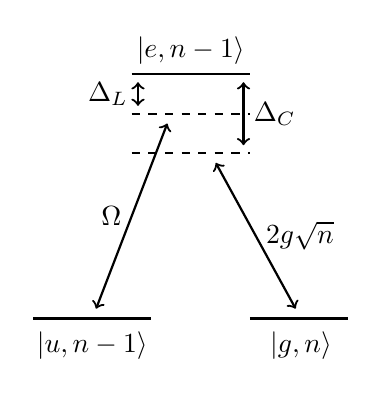
\begin{tikzpicture}
	
	% Energy levels
	\node at (0,3.3)    {$\left|e, n-1\right\rangle$};
	\node at (-1.25,-0.45)   {$\left|u, n-1\right\rangle$};
	\node at (1.4,-0.45)    {$\left|g, n\right\rangle$};
	
	\node at (0,3) (e) {};
	\node at (-1.25,-0.1) (u) {};
	\node at (1.4,-0.1) (g) {};
	\node at (-0.25,2.5) (d1) {};
	\node at (0.25,2) (d2) {};
	
	% Horizontal lines for energy levels
	\draw[thick] (-0.75,3) -- (0.75,3);
	\draw[thick] (-2,-0.1) -- (-0.5,-0.1);
	\draw[thick] (0.75,-0.1) -- (2,-0.1);
	
	% Arrows connecting energy levels
	\draw[thick, <->] (d1) -- node[midway, left] {$\Omega$} (u);
	\draw[thick, <->] (d2) -- node[midway, right] {$2g\sqrt{n}$} (g);
	
	% Dashed lines for detunings
	\draw[thick, dashed] (-0.75,2.5) -- (0.75,2.5);
	\draw[thick, dashed] (-0.75,2) -- (0.75,2);
	
	% Detuning labels
	\draw[thick, <->] (0.67,2.1) -- node[midway, right] {$\Delta_C$} (0.67,2.9);
	\draw[thick, <->] (-0.67,2.6) -- node[midway, left] {$\Delta_L$} (-0.67,2.9);
	
	\end{tikzpicture}
	\caption[Energy level diagram of a $\Lambda$-like three-level system]{Energy level diagram of a $\Lambda$-like three-level system showing the detunings ($\Delta_L$, $\Delta_C$) and Rabi frequencies ($\Omega$, $2g\sqrt{n}$) of the driving field and cavity, respectively.}
	\label{fig:3lvlLambdaSystem}
\end{figure}
Analogous to the two-level system, the Hamiltonian (in the rotating frame) of the three-level system can be decomposed into blocks that now couple the atom-field states $\{\vert u, n-1 \rangle,  \vert e,n-1\rangle, \vert g, n\rangle\}$ as
\begin{align}
\label{hamiltonianHn}
\begin{split}
\hat{\mathcal{H}}_n \begin{pmatrix}  \vert u, n-1 \rangle \\ \vert e, n-1\rangle \\ \vert g, n\rangle \end{pmatrix} = \hbar \begin{pmatrix} n\omega_C & \Omega/2 & 0 \\ \Omega/2 & n\omega_C + \Delta_L & g\sqrt{n} \\ 0 & g\sqrt{n} &  n\omega_C + \Delta_L-\Delta_C \end{pmatrix} \begin{pmatrix} \vert u, n-1 \rangle \\ \vert e, n-1\rangle \\ \vert g, n\rangle \end{pmatrix}\,.
\end{split}
\end{align}
For equal laser and cavity detuning ($\Delta_L=\Delta_C=\Delta$), the eigenfrequencies are given by
\begin{align}
\begin{split}
\omega_{n}^0 &= n\omega_C  \\
\omega_{n}^{\pm} &= n\omega_C + \frac{1}{2} \left(\Delta \pm \sqrt{\Omega_n^2 + \Omega^2 + \Delta^2 } \right)\,,
\label{eq:3lvlTripletEnergies}
\end{split}
\end{align}
with the following corresponding eigenstates:\iffalse \cite{kuhn10} \fi
\begin{align}
\begin{split}
\vert \psi^0_n \rangle &= \cos(\theta_n)\vert u,n-1\rangle - \sin(\theta_n)\vert{g,n}\rangle \\
\vert \psi^+_n \rangle &= \sin(\phi_n)\sin(\theta_n)\vert{u,n-1}\rangle + \cos(\phi_n)\vert{e,n-1}\rangle + \sin(\phi_n)\cos(\theta_n)\vert{g,n}\rangle \\
\vert \psi^-_n \rangle &= \cos(\phi_n)\sin(\theta_n)\vert{u,n-1}\rangle - \sin(\phi_n)\vert{e,n-1}\rangle + \cos(\phi_n)\cos(\theta_n)\vert{g,n}\rangle\,,
\label{eq:3lvlTripletStates}
\end{split}
\end{align}
where $\theta_n$ and $\phi_n$ are the mixing angles defined by
\begin{align}
\tan(\theta_n)=\frac{\Omega}{\Omega_n}\quad
\tan(\phi_n) = \frac{\sqrt{\Omega_n^2 + \Omega^2}}{\sqrt{\Omega_n^2 + \Omega^2 + \Delta^2} + \Delta}\,. 
\label{eq:3lvlTripletStatesMixingAngles}
\end{align}
In the limit of a vanishing laser coupling ($\Omega\rightarrow 0 $), the states $\vert \psi ^\pm _n \rangle $ correspond to the dressed states of the two-level system as defined in \autoref{dressedstates}, while $\vert \psi ^0 _n \rangle $ reduces to $ \vert u, n-1\rangle$. In general, $\vert \psi ^0 _n \rangle$ is referred to as the dark eigenstate, since it involves a linear combination of the grounds states only. Note that the distribution across the ground states depends only on the ratio of the relevant couplings strengths ($\sfrac{\Omega}{\Omega_n}$). This implies that, starting from the state $\vert u, 0\rangle$, the population can be adiabatically transferred between the ground states by means of an adequately shaped control pulse $\Omega(t)$. This process avoids any transient population in the excited state, which suppresses spontaneous emission into free space. As will be discussed in the following section, a realistic cavity is subject to photon loss. This means that, once the system reaches the state $ \vert g, 1\rangle $, the photon will irreversibly decay from the cavity at a constant rate, eventually leaving the system in the state $ \vert g, 0\rangle$. This cavity-mediated, adiabatic population transfer is referred to as Vacuum Stimulated Raman Adiabatic Passage (V-STIRAP) and constitutes a valuable method for extracting and shaping single photons from atoms \cite{Kuhn2002,McKeever2004,Brattke2001}. This is especially relevant for photons in the context of linear optics quantum computing (LOQC) \cite{Knill2001,Ralph2001,Kok2007,OBrien2007}, the scalability of which relies heavily on deterministic single-photon generation and preparation.

\subsection{Loss mechanisms in an atom-cavity system}
In the preceding discussion of the dressed eigenstates of two- and three-level systems, we have ignored the effect of spontaneous emission and cavity field decay. In practice, a good model for a single-mode radiation field is that of an optical cavity, which consists of two reflective mirrors. By trapping an atom inside this cavity, light-matter interaction can be achieved. \autoref{fig:JCFPcavity} illustrates a two-level atom confined within a cavity with mode volume $V$.
\begin{figure}[t]
	\centering
	\begin{tikzpicture}
	
	% Colors
	\definecolor{cavitycolor}{RGB}{244,177,157}
	\definecolor{cylindercolor}{RGB}{154,182,206}
	\definecolor{atomcolor}{RGB}{255,238,214}
	
	\def\a{(0, 2) circle (1.4)}
	\def\b{(0, 0) circle (2)}
	\def\c{(0, -2) circle (1.4)}
	
	\begin{scope}
	\clip \b;
	\clip[reverseclip] \a;
	\clip[reverseclip] \c;
	\fill[cavitycolor,even odd rule] \a \b \c;
	\end{scope}
	
	\def\A{(-2.5,2) to[out=0,in=180] (-1,2) -- (-1,-2) to[out=180,in=0] (-2.5,-2) -- cycle};
	\def\B{(2.5,2) to[out=180,in=0] (1,2) -- (1,-2) to[out=0,in=180] (2.5,-2) -- cycle};
	\def\C{(0.2,2) arc[start angle=90, end angle=270, radius=2cm] -- cycle};
	\def\D{(-0.2,-2) arc[start angle=-90, end angle=90, radius=2cm] -- cycle};
	
	\def\E{(-2,2) to[out=0,in=180] (2,2) -- (2,-2) to[out=180,in=0] (-2,-2) -- cycle};
	\def\F{(0,1) arc[start angle=0, end angle=180, radius=2cm] -- cycle};
	% Draw cavity
	%\fill[cavitycolor] (-2,2) to[out=0,in=180] (2,2) -- (2,-2) to[out=180,in=0] (-2,-2) -- cycle;
	
	
	\begin{scope}
	\clip \A;
	\clip[reverseclip] \C;
	\fill[cylindercolor, draw=none, even odd rule] \C \A \D;
	\end{scope}
	
	\begin{scope}
	\clip \B;
	\clip[reverseclip] \D;
	\fill[cylindercolor, even odd rule] \C \B \D;
	\end{scope}
	
	
	% Draw atom
	\fill[atomcolor] (0,0) circle (0.4);
	\draw[thick] (-0.15,0.15) -- (0.15,0.15);
	\draw[thick] (-0.15,-0.15) -- (0.15,-0.15);
	\draw[fill=atomcolor] (0,0.15) circle (0.05);
	\fill (0,-0.15) circle (0.05);
	\centerarc[->,thick](0.61,0)(5:155:0.4);
	\centerarc[->,thick](0.61,0)(210:355:0.4);
	\node[anchor=center] at (0.61,-0.02) {$g$};
	
	% Photon emission
	\draw[->,thick,decorate,decoration={snake,amplitude=.4mm,segment length=2mm}] (-0.2,-0.2) -> (-0.65,-1.23);
	\node at (-0.3,-1.2) {$\gamma$};
	
	% Cavity photon decay
	\draw[thick,->] (2,0) -- (3,0);
	\node at (2.75,0.2) {$\kappa$};
	
	% Energy level diagram
	\fill[atomcolor] (6,0) circle (2);
	\draw[thick] (5,-1) -- (6.5,-1);
	\draw[thick] (5,1) -- (6.5,1);
	\draw[thick,dashed] (5.5,0.4) -- (6.5,0.4);
	
	\draw[thick,dashed, atomcolor] (-0.1,0.38) -- (5.7,1.96);
	\draw[thick,dashed, atomcolor] (-0.1,-0.38) -- (5.7,-1.96);
	
	% Energy levels labels
	\draw[<->, thick] (5.2,-0.95) -- (5.2,0.95) node[midway, left] {$\omega_{0}$};
	\draw[<->, thick] (5.7,-0.95) -- (5.7,0.35) node[midway, right] {$\omega$};
	\draw[<->, thick] (5.7,0.95) -- (5.7,0.45) node[midway, right] {$\Delta$};
	
	\node at (7,1) {$|e\rangle$};
	\node at (7,-1) {$|g\rangle$};
	
	
	\end{tikzpicture}
	\caption[Coupling and decay channels in an atom-cavity system]{The atom-cavity system shown on the left is characterised by the coupling strength $g$, the field decay rate from the cavity $\kappa$ and the amplitude decay rate of the atomic state $\gamma$. The energy level diagram of the two-level atom is shown on the right. The ground and excited states $\vert{g}\rangle$ and $\vert{e}\rangle$ are separated by a frequency $\omega_{0}$. The cavity, which operates at a frequency $\omega$, is detuned from the atomic resonance by $\Delta$.}
	\label{fig:JCFPcavity}
\end{figure}
The atom-cavity system is characterised by three key parameters: $g$, $\kappa$, and $\gamma$, which represent the atom-cavity coupling strength, the field decay rate from the cavity and the transverse polarisation decay rate\footnote{In the radiative limit, the transverse polarisation decay rate (loss of coherence or dephasing) equals half the population relaxation rate: $\gamma=\sfrac{\Gamma}{2}$. In general, $\gamma=\sfrac{\Gamma}{2}+\gamma_\phi$, where $\gamma_\phi$ is the pure dephasing rate, which describes the loss of coherence due to environmental interactions, without population transfer occurring between states.} of the atom, respectively. The interaction between the atom and the radiation field intensifies if the cavity is resonant with the atomic transition ($\Delta=0$), a condition that is achieved by adjusting the cavity length so that the frequency $\omega$ of the cavity mode matches $\omega_0$. The photon decay rate $\kappa$ depends on the properties of the cavity and is related to its quality factor $Q$ via the relation
\begin{align}
\label{qfactor}
	Q = \frac{\omega}{2\kappa}\,.
\end{align}
Note that $\sfrac{1}{2\kappa}$ represents the time over which the average stored energy in the cavity decreases to $\sfrac{1}{\mathrm{e}}$ of its original value. If follows from \autoref{qfactor} that a high $Q$ factor corresponds to a relatively low photon decay rate. The transverse polarisation decay rate $\gamma$ is affected by several factors. For instance, an atom may emit a photon at the resonant frequency in a direction that does not align with the cavity mode. Alternatively, the atom could transition to other energy levels, resulting in the emission of a photon with a different frequency that is not resonant with the cavity. The effect of spontaneous emission on the vacuum Rabi oscillations in a three-level system as in \autoref{fig:3lvlLambdaSystem} is shown in \autoref{fig:VacuumRabiOscillations}. The population oscillates between the states $\vert e, 0 \rangle$ and $\vert g, 1 \rangle$, whilst energy dissipates from the system as a result of spontaneous emission.
\begin{figure}[!t]
	%\vspace{0.7em}
	\centering
	\begin{tikzpicture}
	\begin{groupplot}[group style={group size=2 by 1, horizontal sep=2.5cm},height=5.5cm,width=5.5cm,no markers]
	\nextgroupplot
	[
	%title={Temperature dependence of CuSO$_4\cdot$5H$_2$O solubility},
	xlabel={Time ($\mu$s)},
	ylabel={Photon number $\langle \hat{n} \rangle$},
	xmin=0, xmax=0.2,
	ymin=0, ymax=0.8,
	xticklabels={0,0.05,0.1,0.15,0.2},
	xtick={0,0.05,0.1,0.15,0.2},
	%legend pos=north west,
	ymajorgrids=true,
	xmajorgrids=true,
	grid style=dashed,
	]
	
	\addplot[
	color=markrood,
	/pgfplots/error bars/.cd,
	x dir = both,
	x explicit,
	] table [col sep = comma, x index = 0, y expr=\thisrowno{1}]{VRO_get_cavity_number.csv};
	
	\nextgroupplot
	[
	%title={Temperature dependence of CuSO$_4\cdot$5H$_2$O solubility},
	xlabel={Time ($\mu$s)},
	ylabel={Atomic state population},
	xmin=0, xmax=0.2,
	ymin=0, ymax=1.0,
	xticklabels={0,0.05,0.1,0.15,0.2},
	xtick={0,0.05,0.1,0.15,0.2},
	%legend pos=north west,
	ymajorgrids=true,
	xmajorgrids=true,
	grid style=dashed,
	legend cell align={left},
	legend style={
		at={(1, 1)},  % Adjust (x, y) to move it
		anchor=north east,  % Attach the legend to its top-right corner
		draw=none,           % Optional: Remove border around the legend
		fill=none
	}
	%legend pos=north east,
	%legend cell align={left},
	%legend style={draw=none,fill=none,text opacity=1},
	]
	
	\addplot[
	color=rainbow1of8,
	/pgfplots/error bars/.cd,
	x dir = both,
	x explicit,
	] table [col sep = comma, x index = 0, y expr=\thisrowno{1}]{VRO_get_atomic_population.csv};
	
	\addplot[
	color=rainbow2of8,
	/pgfplots/error bars/.cd,
	x dir = both,
	x explicit,
	] table [col sep = comma, x index = 0, y expr=\thisrowno{4}]{VRO_get_atomic_population.csv};
	
	\addplot[
	color=rainbow3of8,
	/pgfplots/error bars/.cd,
	x dir = both,
	x explicit,
	] table [col sep = comma, x index = 0, y expr=\thisrowno{3}]{VRO_get_atomic_population.csv};
	
	\addlegendentry{\footnotesize \hspace{0.3em} $\vert u \rangle$}
	\addlegendentry{\footnotesize \hspace{0.3em} $\vert e \rangle$}
	\addlegendentry{\footnotesize \hspace{0.3em} $\vert g \rangle$}
	
	\end{groupplot}
	
	\end{tikzpicture}
	\caption[Vacuum Rabi oscillations under the effect of spontaneous emission]{Vacuum Rabi oscillations under the effect of spontaneous emission shown in terms of the expected cavity photon number (left) and atomic state populations (right) as a function of time for a three level system as shown in \autoref{fig:3lvlLambdaSystem}. The initial state of the system is $\vert e, 0 \rangle$ and both the cavity decay rate and driving laser amplitude are set to zero. The atom-cavity coupling strength and transverse polarisation decay rate are given by $(g,\gamma)=2\pi\times(15,3)\,$MHz. The amount of energy dissipated in the form of spontaneously emitted photons lost to the environment amounts to \SI{85}{\percent} of a single excitation.}
	\label{fig:VacuumRabiOscillations} 
\end{figure}

\subsection{Strong coupling regime}
Different coupling regimes exist for the atom-cavity system, the first being the strong coupling regime, in which $g \gg \max \{\kappa,\gamma\}$. In the strong coupling regime, the atom-photon interaction occurs more rapidly than the irreversible processes caused by photon loss from the cavity mode. This makes the emission of the photon a reversible process, where the photon is reabsorbed by the atom before it escapes the cavity, resulting in vacuum Rabi oscillations. Another way in which this regime can be characterised is via the cooperativity $C$, which is defined as
\begin{align}
	C=\frac{g^2}{2\kappa\gamma}\,.
\end{align} 
Strong coupling in the atom-cavity system is achieved when $C$ is maximised, a criterion that can be understood in the context of the Purcell factor $F=2C$, which equals the ratio of emission into the cavity ($\sfrac{g^2}{\kappa}$) to the spontaneous emission probability into free space ($\gamma$). Experimentally, strong coupling typically occurs in cavities with a small mode volume $V$ and minimal losses (high $Q$). Early demonstrations of the strong coupling limit in CQED were based on a variety of physical systems. These include alkali atoms in an optical Fabry--P\'{e}rot cavity \cite{Thompson1992}, Rydberg atoms in a microwave cavity \cite{Brune1996}, superconducting qubits coupled to on-chip microwave resonators \cite{Wallraff2004} or superconducting quantum interference devices \cite{Chiorescu2004}, and semiconductor quantum dots coupled to photonic crystals \cite{Yoshie2004} or micropillar resonators \cite{Reithmaier2004}.

In the strong coupling regime, where the energy exchange between atom and cavity is fast and coherent, the method of V-STIRAP (as discussed in \autoref{vstirap}) can be employed to adiabatically transfer the population between $\vert u, 0\rangle$ and $\vert g, 1\rangle$ via an adequately shaped control pulse $\Omega(t)$. This process is shown in \autoref{fig:StrongCoupling}. A larger detuning suppresses the transient population in the excited state and therefore reduces the amount of spontaneous emission into free space. Photon generation efficiencies in the strong coupling regime can therefore reach values close to unity. However, if the cavity decay rate is much larger than the coupling strength (as will be discussed in the following section), photons leak out of the cavity too quickly and the system cannot maintain coherence over the time needed for the V-STIRAP process.
\begin{figure}[!t]
	%\vspace{0.7em}
	\centering
	\begin{tikzpicture}
	\begin{groupplot}[group style={group size=2 by 1, horizontal sep=2.5cm},height=5.5cm,width=5.5cm,no markers]
	\nextgroupplot
	[
	%title={Temperature dependence of CuSO$_4\cdot$5H$_2$O solubility},
	xlabel={Time ($\mu$s)},
	ylabel={Cavity emission rate ($\mu$s$^{-1}$)},
	xmin=0, xmax=2,
	ymin=0, ymax=2,
	%xticklabels={0,0.1,0.2,0.3},
	%xtick={0,0.1,0.2,0.3},
	%legend pos=north west,
	ymajorgrids=true,
	xmajorgrids=true,
	grid style=dashed,
	samples=200
	]
	
	\addplot[markgrijs, dashed] {(sin(deg(pi*x/(2))))^2};
	
	\node[markgrijs] at (1.6,0.8) {\footnotesize $\Omega(t)$};
	
	\addplot[
	color=markrood,
	/pgfplots/error bars/.cd,
	x dir = both,
	x explicit,
	] table [col sep = comma, x index = 0, y expr=\thisrowno{1}]{SCR_get_cavity_emission.csv};
	
	\nextgroupplot
	[
	%title={Temperature dependence of CuSO$_4\cdot$5H$_2$O solubility},
	xlabel={Time ($\mu$s)},
	ylabel={Atomic state population},
	xmin=0, xmax=2,
	ymin=0, ymax=1.0,
	%xticklabels={0,0.1,0.2,0.3},
	%xtick={0,0.1,0.2,0.3},
	%legend pos=north west,
	ymajorgrids=true,
	xmajorgrids=true,
	grid style=dashed,
	legend cell align={left},
	legend style={
		at={(1, 0.9)},  % Adjust (x, y) to move it
		anchor=north east,  % Attach the legend to its top-right corner
		draw=none,           % Optional: Remove border around the legend
		fill=none
	}
	%legend pos=north east,
	%legend cell align={left},
	%legend style={draw=none,fill=none,text opacity=1},
	]
	
	\addplot[
	color=rainbow1of8,
	/pgfplots/error bars/.cd,
	x dir = both,
	x explicit,
	] table [col sep = comma, x index = 0, y expr=\thisrowno{1}]{SCR_get_atomic_population.csv};
	
	\addplot[
	color=rainbow2of8,
	/pgfplots/error bars/.cd,
	x dir = both,
	x explicit,
	] table [col sep = comma, x index = 0, y expr=\thisrowno{4}]{SCR_get_atomic_population.csv};
	
	\addplot[
	color=rainbow3of8,
	/pgfplots/error bars/.cd,
	x dir = both,
	x explicit,
	] table [col sep = comma, x index = 0, y expr=\thisrowno{3}]{SCR_get_atomic_population.csv};
	
	\addlegendentry{\footnotesize \hspace{0.3em} $\vert u \rangle$}
	\addlegendentry{\footnotesize \hspace{0.3em} $\vert e \rangle$}
	\addlegendentry{\footnotesize \hspace{0.3em} $\vert g \rangle$}
	
	\end{groupplot}
	
	\end{tikzpicture}
	\caption[Time evolution of a three-level atom-cavity system in the strong coupling regime]{Time evolution of the cavity emission rate (left) and atomic state populations (right) for a three level system (\autoref{fig:3lvlLambdaSystem}) in the strong coupling regime. The driving pulse has a temporal profile of $\Omega(t)=g\sin^2(\pi t/\SI{2}{\micro\second})$ and is shown as a dashed line on the left. The initial state of the system is $\vert u, 0 \rangle$ and the relevant parameters are given by $\Delta_L=\Delta_C=0$ and $(g,\gamma,\kappa)=2\pi\times(15,3,2)\,$MHz. The total photon emission probability from the cavity is \SI{95}{\percent} and the amount of energy dissipated in the form of spontaneously emitted photons lost to the environment amounts to \SI{5.4}{\percent} of a single excitation.}
	\label{fig:StrongCoupling} 
\end{figure}

\subsection{Dynamics in the bad-cavity regime}
In addition to the strong coupling regime, we consider the dynamics in bad-cavity regime, which is characterised by $\kappa \gg \sfrac{g^2}{\kappa} \gg \gamma $. Let us assume that the atom is excited with a pump pulse, while it emits a photon into the cavity via enhanced spontaneous emission. In this case, the bad cavity regime implies that the fastest timescale is set by the cavity field decay, while the spontaneous emission rate into the cavity dominates the incoherent polarisation decay of the atom, where the excitation is lost to unwanted modes of the radiation field. Quantitatively, the dynamics of a three-level system consisting of the states $\{ \vert u, 0 \rangle, \vert e, 0 \rangle, \vert g, 1 \rangle \}$ as described in the preceding section can be found by solving the Schr\"{o}dinger equation for the coefficients in the time dependent state vector $\vert \psi (t) \rangle = c_u(t)\vert u,0\rangle+c_e(t)\vert e, 0 \rangle + c_g(t) \vert g,1\rangle$. To this end, we employ the non-Hermitian Hamiltonian
\begin{align}
	\hat{\mathcal{H}}' = \hat{\mathcal{H}}_1 - i \hbar (\kappa \hat{a}^\dagger\hat{a}+\gamma \vert e \rangle\langle e \vert)\,,
\end{align}
which includes the Hermitian Hamiltonian $\hat{\mathcal{H}}_1$ as defined in \autoref{hamiltonianHn} and two additional terms that describe the cavity field decay and spontaneous emission. Assuming that $\Delta_L=\Delta_C=0$ and that the initial state is $\vert u, 0\rangle$, one can find an adiabatic solution as long as $\Omega(t)\ll \sfrac{g^2}{\kappa}$. This condition implies that the rate of spontaneous emission into the cavity is sufficiently fast to ensure that the populations in $\vert e,0\rangle$ and $\vert g, 1 \rangle$ are nearly time independent ($\dot{c}_e(t)\approx 0 $ and $\dot{c}_g(t)\approx 0$). Solving for $c_g(t)$, we obtain
\begin{align}
	c_g(t)\approx-\frac{g}{2\kappa} \alpha \Omega(t) \exp{-\frac{\alpha}{4} \int_{0}^{t} \Omega^2(\tau) \mathrm{d}\tau}\,,
\end{align} 
where the constant $\alpha$ is defined as $\alpha=\frac{1}{\gamma+\sfrac{g^2}{\kappa}}$. This implies that the photon emission from the cavity occurs at a rate of $2\kappa \vert c_g(t)\vert^2$, since $\vert g, 1 \rangle$ is the only state from which the system can decay to $\vert g, 0 \rangle$ via the emission of a photon. The total photon emission probability $\eta$ therefore equals
\begin{align}
 \eta = \int 2\kappa \vert c_g(t)\vert^2 \mathrm{d}t=\frac{g^2}{\kappa}\alpha \left( 1 -  \exp{-\frac{\alpha}{2} \int \Omega^2(t) \mathrm{d}t} \right)\,.
\end{align}
Note that the exponential term vanishes for a sufficiently large pulse area, which leads to a simplified emission probability of
\begin{align}
\eta\approx \frac{g^2}{\kappa}\alpha = \frac{2C}{2C+1}\,,
\end{align}
written in terms of the cooperativity. In the bad cavity regime, photon generation efficiencies are typically lower compared to the strong coupling regime, since part of the population is placed in the excited state, which results in unavoidable spontaneous emission into modes other than the cavity mode (see \autoref{fig:BadCavityRegime}).
\begin{figure}[h]
	%\vspace{0.7em}
	\centering
	\begin{tikzpicture}
	\begin{groupplot}[group style={group size=2 by 1, horizontal sep=2.5cm},height=5.5cm,width=5.5cm,no markers]
	\nextgroupplot
	[
	%title={Temperature dependence of CuSO$_4\cdot$5H$_2$O solubility},
	xlabel={Time ($\mu$s)},
	ylabel={Cavity emission rate ($\mu$s$^{-1}$)},
	xmin=0, xmax=0.3,
	ymin=0, ymax=9,
	%xticklabels={0,0.1,0.2,0.3},
	%xtick={0,0.1,0.2,0.3},
	%legend pos=north west,
	ymajorgrids=true,
	xmajorgrids=true,
	grid style=dashed,
	samples=1000
	]
	
	\addplot[markgrijs, dashed] {4.5*(sin(deg(pi*x/(0.3))))^2};
	
	\node[markgrijs] at (0.26,3) {\footnotesize $\Omega(t)$};
	
	\addplot[
	color=markrood,
	/pgfplots/error bars/.cd,
	x dir = both,
	x explicit,
	] table [col sep = comma, x index = 0, y expr=\thisrowno{1}]{BCR_get_cavity_emission.csv};
	
	\nextgroupplot
	[
	%title={Temperature dependence of CuSO$_4\cdot$5H$_2$O solubility},
	xlabel={Time ($\mu$s)},
	ylabel={Atomic state population},
	xmin=0, xmax=0.3,
	ymin=0, ymax=1.0,
	%xticklabels={0,0.1,0.2,0.3},
	%xtick={0,0.1,0.2,0.3},
	%legend pos=north west,
	ymajorgrids=true,
	xmajorgrids=true,
	grid style=dashed,
	legend style={
		at={(1, 0.75)},  % Adjust (x, y) to move it
		anchor=north east,  % Attach the legend to its top-right corner
		draw=none,           % Optional: Remove border around the legend
		fill=none
	}
	%legend pos=north east,
	%legend cell align={left},
	%legend style={draw=none,fill=none,text opacity=1},
	]
	
	\addplot[
	color=rainbow1of8,
	/pgfplots/error bars/.cd,
	x dir = both,
	x explicit,
	] table [col sep = comma, x index = 0, y expr=\thisrowno{1}]{BCR_get_atomic_population.csv};
	
	\addplot[
	color=rainbow2of8,
	/pgfplots/error bars/.cd,
	x dir = both,
	x explicit,
	] table [col sep = comma, x index = 0, y expr=\thisrowno{4}]{BCR_get_atomic_population.csv};
	
	\addplot[
	color=rainbow3of8,
	/pgfplots/error bars/.cd,
	x dir = both,
	x explicit,
	] table [col sep = comma, x index = 0, y expr=\thisrowno{3}]{BCR_get_atomic_population.csv};
	
	\addlegendentry{\footnotesize \hspace{0.3em} $\vert u \rangle$}
	\addlegendentry{\footnotesize \hspace{0.3em} $\vert e \rangle$}
	\addlegendentry{\footnotesize \hspace{0.3em} $\vert g \rangle$}
	
	\end{groupplot}
	
	\end{tikzpicture}
	\caption[Time evolution of a three-level atom-cavity system in the bad cavity regime]{Time evolution of the cavity emission rate (left) and atomic state populations (right) for a three level system (\autoref{fig:3lvlLambdaSystem}) in the bad cavity regime. The driving pulse has a temporal profile of $\Omega(t)=g\sin^2(\pi t/\SI{2}{\micro\second})$ and is shown as a dashed line on the left. The initial state of the system is $\vert u, 0 \rangle$ and the relevant parameters are given by $\Delta_L=\Delta_C=0$ and $(g,\gamma,\kappa)=2\pi\times(15,3,20)\,$MHz. The total photon emission probability from the cavity is \SI{76}{\percent} and the amount of energy dissipated in the form of spontaneously emitted photons lost to the environment amounts to \SI{41}{\percent} of a single excitation.}
	\label{fig:BadCavityRegime} 
\end{figure}
However, it is still possible to achieve reasonable efficiencies given adequate values for $g$, $\kappa$ and $\alpha$. In this regime, the cavity serves more as a filter or a channel to direct the photon into a particular mode, but it does not significantly enhance the emission process. The photon leaks out quickly from the cavity because the cavity’s lifetime is short and the temporal profile of its wavepacket can be controlled via the pulse shape $\Omega(t)$. While less efficient than the strong coupling regime, the bad cavity regime can be easier to implement in practice, as it puts less stringent requirements on the atom-cavity coupling and mirror reflectivity.

\end{document}
